
\begin{figure}[H]
    \centering
    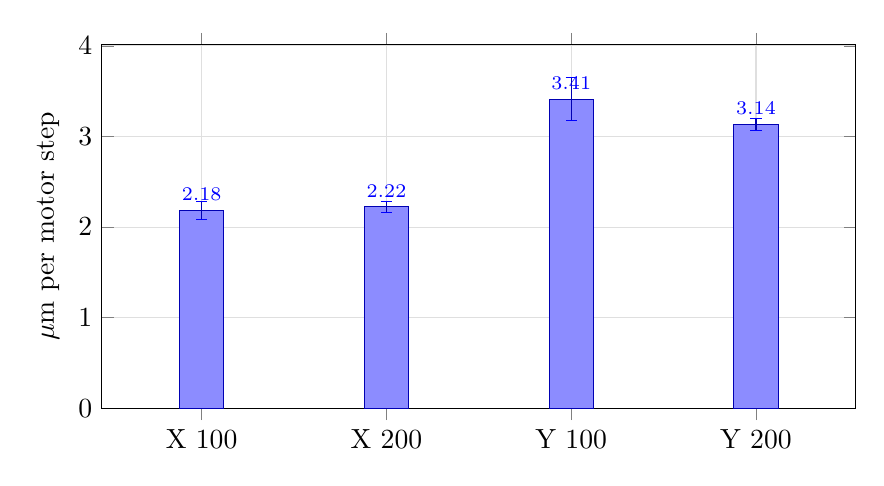
\begin{tikzpicture}
        \begin{axis}[
            width=0.92\linewidth,
            height=6.2cm,
            ybar,
            bar width=16pt,
            ymin=0,
            ylabel={$\mu$m per motor step},
            symbolic x coords={X100,X200,Y100,Y200},
            xtick=data,
            xticklabels={X 100,X 200,Y 100,Y 200},
            nodes near coords,
            nodes near coords align={vertical},
            every node near coord/.append style={font=\scriptsize},
            error bars/y dir=both, error bars/y explicit,
            enlarge x limits=0.18,
            grid=major,
            major grid style={draw=gray!25},
        ]
        \addplot+[fill=blue!45, draw=blue!70!black] coordinates {
            (X100,2.1832) +- (0,0.0952)
            (X200,2.2229) +- (0,0.0575)
            (Y100,3.4099) +- (0,0.2379)
            (Y200,3.1358) +- (0,0.0665)
        };
        \end{axis}
    \end{tikzpicture}
    \caption[4x stage-scale repeatability plot]{Stage-scale repeatability for a 4x objective. Bars show the mean stage scale and error bars show standard deviation across ten valid trials per condition (X and Y, 100 and 200 steps).}
    \label{fig:eval-stage-scale}
\end{figure}
